% !TeX spellcheck = en_US
\section{System Architecture}
\noindent A graphical representation of the system architecture can be seen in figure \ref{fig:architecture}.

\begin{figure}[H]
	\centering
	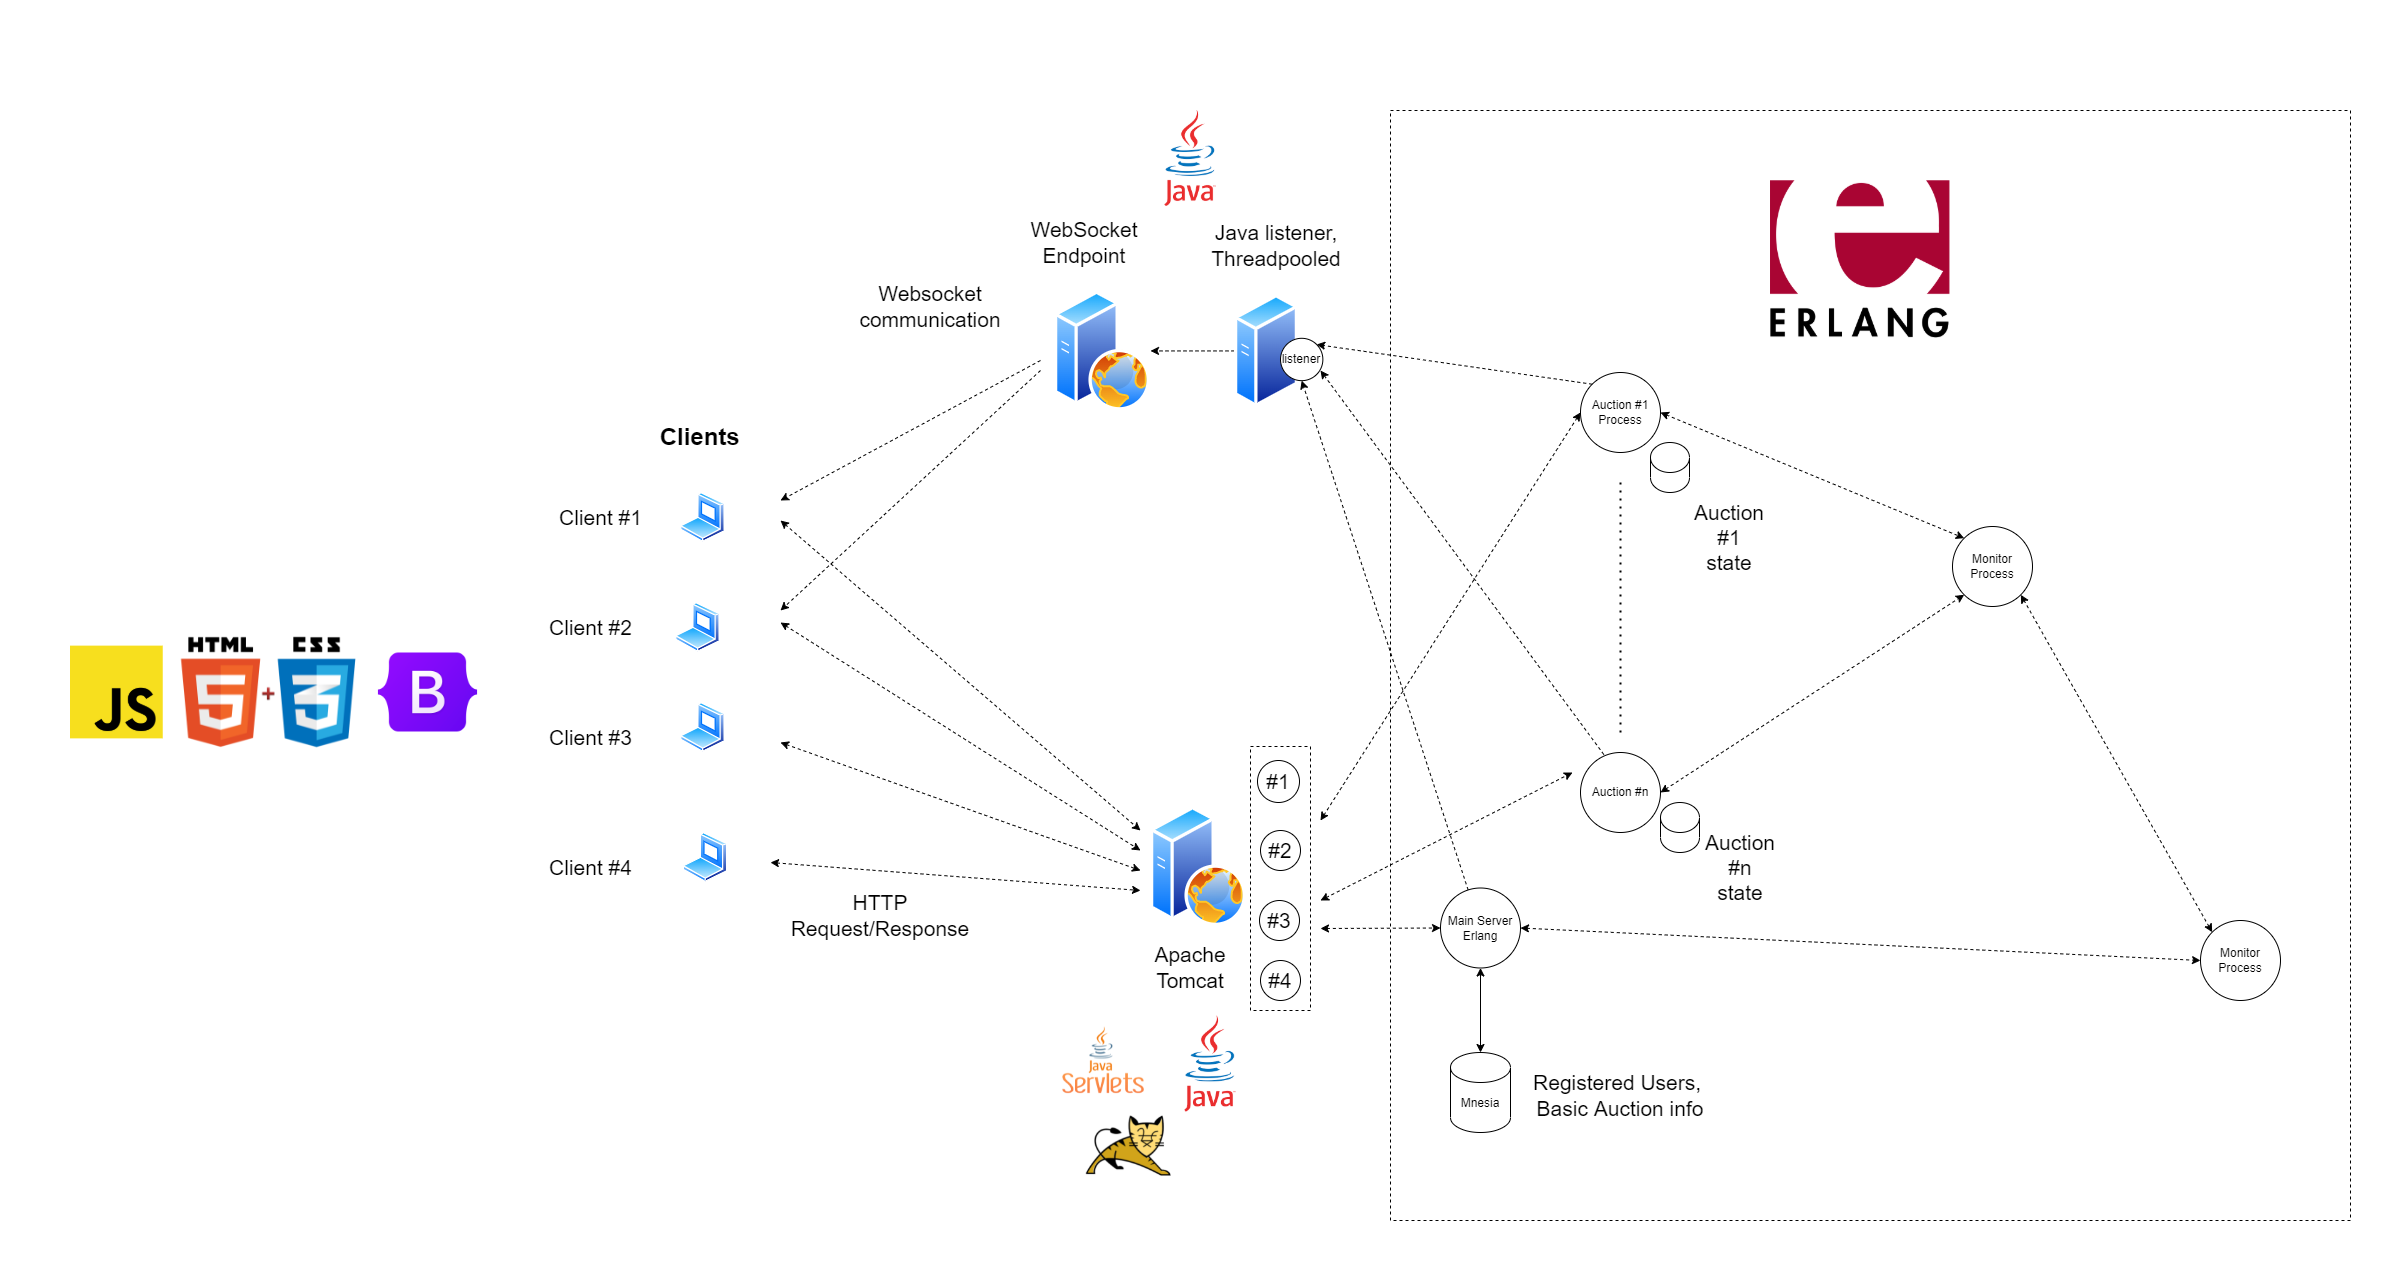
\includegraphics[width=1\linewidth]{img/systemStructure2.png}
	\caption{System Architecture graphical representation}
	\label{fig:architecture}
\end{figure}

\noindent We can divide the overall system in two part:
\begin{itemize}
	\item The server side part: developed in Erlang, it is in charge of handling the request coming from the users and it has to handle the auctions and to maintain the global view of an auctions consistent among the users.
	
	\item The client side part: developed in Java, using Servlets and JSP for handling HTTP requests, content generation and websocket endpoint, and in Javascript for what concern the handling of websocket messages. It is in charge of retrieving information from the server, creating the GUI, updating the GUI in order to let the user have a consistent view of the state of the auction and of the overall system.
\end{itemize}

\noindent The server-side part written in Erlang and the Java Listener are deployed in the container \textbf{172.18.0.7}, Apache Tomcat webserver which hosts the Web Application is deployed in the container \textbf{172.18.0.6}.
Is possible to access those containers by using OpenVPN with the file \textit{studenti.ovpn} that can be found
in the main project repository: \\
\url{https://github.com/gerti98/DistributedSystemsProject}
	
\noindent The Web-App can be accessed through the following link: \\ \url{http://172.18.0.6:8080/AuctionHandlerWebApp/LoginServlet}

\subsection{Server Side}
\noindent The Server side part is written in Erlang and contains the following components:

\begin{itemize}
	\item The Main Server
	\item Auction Handler
	\item Auctions Monitor
	\item Supervisor
	\item MnesiaDB
\end{itemize}

\subsubsection{Main Server}
\noindent The main server is in charge of receiving requests from the client side and saving all the necessary information in the database.

\noindent Since robustness is required the main server is an OTP gen\_server. The main server is actually composed by an endpoint and by the actual server. The endpoint is a sort of API used to make a call to the OTP gen\_server:
\begin{enumerate}
	\item The client sends a message to the endpoint
	\item The endpoint receives the message, analyzes it and calls the function that uses the function call in order to make a request to the OTP gen\_server
	\item The OTP gen\_server receives the request and calls the function handle\_call that matches with the incoming message pattern.
	\item The handle\_call function will manage the request arrived from the client and sent back the required information (saving info in the database or spawning process if necessary)
\end{enumerate}
\noindent The functionalities that the server exposes are:
\begin{itemize}
	\item Register a new user
	
	\noindent The user will be registered (i.e. added to the database) if and only if its username is not already present in the database.
	
	\item Login
	
	\noindent The username and password are checked and if both are correct a positive reply is sent back
	
	\item Create Auction
	
	\noindent A new auction is created (added to the database) if and only if another auction with the same name is not already present in the database. When the auction is created a new process (i.e. The Auction Handler) is spawned and this process is added to the processes that the Auctions Monitor has to monitor (for more detail about the monitoring see \ref{Monitoring}).
	From now on for all the information regarding that auction the client has to contact the auction handler at the pid present in the reply message.
	
	\item Retrieve Auction PID
	
	\noindent Return back to the user the PID of the handler that manages the auction with the name passed to the server in the payload of the request. This is very useful for instance when the auction handler crashes and it is re-spawned. In that cases the PID changes and so the client has to know the new one.
	
	\item Retrieve Active Auctions
	
	\noindent Return back the list of all the active auctions (They are saved in the database).
	
	\item Retrieve Passed Auctions
	
	\noindent Return back the list of all the passed auctions (They are saved in the database).
	
	\item Update Win
	
	\noindent Save the username of the auction's winner. This functionality is used by the auction handler in order to store in the persistent storage the name of the winner.
	
	\item Update PID
	
	\noindent Change the PID of the auction handler associated to a particular auction. This is used by the auction monitor when an auction handler crashes and so it is re-spawned with a new PID.
\end{itemize}


\subsubsection{Auction Handler}
\noindent The auction handler's role is to manage an auction maintaining its state.
Its functionalities are:

\begin{itemize}
	\item Maintain the time that remains for the end of the auction.
	
	\noindent Each seconds a clock message is sent by the auction handler to itself in order to emulate the passing time. When the remaining time is 0 (the information about the remaining time are kept into the handler state) then the auction handler has to decide the winner. After this decision the handler kills itself.
	
	\item Remember which users are online at any moment
	
	\noindent Each time a new user enters the auction or leave it, we update the handler state and we notify the client through the Java Listener. 
	
	\item Register the offers
	
	\noindent When a new offer arrives the handler saves it into an ordered list\footnote{The list is composed by tuples e.g. \{"UserA",10\}} (the higher offers is at the beginning of the list) in its internal state. Notice that the offer is registered only if the offer amount is higher w.r.t. the minimal amount.
	
	
	\item Decide the winner
	
	\noindent The winner is the one whose offer is in the first position in the list of the offers. If the list is empty then this means that no offers have been made and so there is no winner. When the winner is decided the client and the main server are notified.
	\noindent
\end{itemize}

\subsubsection{Monitor And Supervisor} \label{Monitoring}
\noindent It is possible to see a graphical representation of the monitoring relationships among processes in figure \ref{fig:monitor}. \noindent The monitoring is performed by \textbf{My Supervisor} and \textbf{Auctions Monitor}.

\begin{figure}[H]
	\centering
	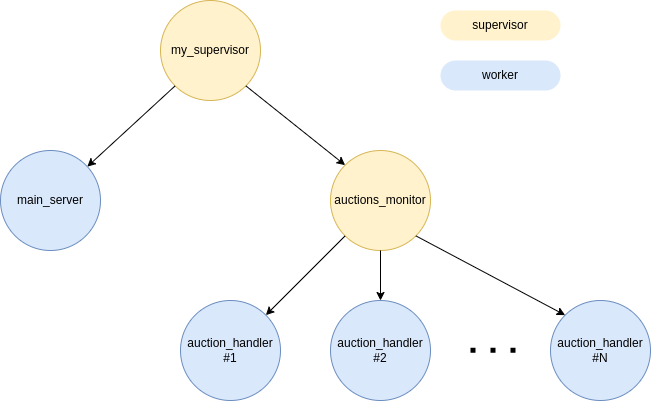
\includegraphics[width=0.7\linewidth]{img/monitorAndSupervisor.png}
	\caption{Graphical representation of how the monitoring is implemented. Notice that in the draw the arrow starts from the monitoring process and ends to the monitored process.}
	\label{fig:monitor}
\end{figure}

%\vspace{0.5cm}

\textbf{My supervisor} is the main supervisor and due to its importance and the robustness required is developed using an OTP supervisor behaviour. The process that it monitors are main\_server and the auctions monitor, both of them are \textit{permanent}. A monitored process is said to be permanent if it is always restarted when necessary.
	
\noindent The restart strategy is \textit{one\_for\_one} since with this stratey we are able to provide the service even if one between main server and auctions monitor crashes. One for one means that if one of the monitored process crashes then only the crashed one is restarted. In our scenario we can have two possibilities:

\begin{itemize}
	\item Main Server crashes
	
	\noindent If the main server crashes before the auction monitor we can just restart it and we have no side effect.
	
	\item Auctions Monitor crashes
	
	\noindent If the auctions monitor crashes and it is restarted then all the auctions created before the crash are not monitored anymore. Anyway that auctions are still reachable by the user and, moreover, the situation is temporary and when the old auctions are terminated we have the standard situation in which all the auctions handler are monitored.
\end{itemize}

\noindent Thus as we can see with this strategy in both cases we are still able to provide the correct service.

\vspace{0.5cm}

\textbf{The auctions monitor} is a custom monitor which is in charge of restart an auction handler when it crashes. To do so it saves in its internal state all the necessary info, in this way when a process crashes abnormally, the auctions monitor restart it and it notifies the main server in order to update the pid with the pid of the new re-spawned auction handler.

\noindent Notice that when the auction handler is re-spawned the state of the auction is the initial one (the state we would have just after the creation of the auction).

\noindent Another thing to highlight is that if the auction handler terminates correctly the auctions monitor does nothing. In fact each auction handler kills itself when the auction ends.


\subsubsection{MnesiaDB}
\noindent The module MnesiaDB is the one in charge of managing the persistent storage. Mnesia has three options regarding the storage persistence (the following three definition are taken from the documentation\footnote{https://www.erlang.org/doc/man/mnesia.html}):
\begin{itemize}
	\item \textit{ram\_copies}. A table can be replicated on a number of Erlang nodes. Property ram\_copies specifies a list of Erlang nodes where RAM copies are kept. These copies can be dumped to disc at regular intervals. However, updates to these copies are not written to disc on a transaction basis.
	
	\item \textit{disc\_copies}. This property specifies a list of Erlang nodes where the table is kept in RAM and on disc. All updates of the table are performed in the actual table and are also logged to disc. If a table is of type disc\_copies at a certain node, the entire table is resident in RAM memory and on disc. Each transaction performed on the table is appended to a LOG file and written into the RAM table.
	
	\item \textit{disc\_only\_copies}. Some, or all, table replicas can be kept on disc only. These replicas are considerably slower than the RAM-based replicas.
\end{itemize}

\noindent The option chosen is \textit{disc\_copies} since makes the database resilient against crashes and allow us to restart the processes without issues. Moreover since the database is kept also on RAM we have also quicker operations (w.r.t. the case disc\_only\_copies). 

\vspace{0.5cm}

\noindent In the database there are two tables:
\begin{itemize}
	\item User
	
	\noindent The attribute of this table are \textit{name} and \textit{password}. It is in charge of remember the users registered to the application.
	
	\item Auction
	
	\noindent The attribute of this table are \textit{name, duration, startingValue, imageURL, creator, pid, winner}.
	It is in charge of remember all the info regarding an auction. An important attribute is \textit{winner}, this attribute is used to distinguish between passed auction and active auction: if the auction is active winner is equal to none, instead if the auction is finished, winner contains a string with the name of the winner or a particular string indicated that there is no winner (if the auctions has received no offers).
\end{itemize}

\noindent A particular feature of Mnesia db is the possibility to use \textit{Atomic transactions}. An atomic transaction ensures that all the operations inside the transaction are performed in an atomic way. This feature is used for the user registration and for auction creation. In both cases we need to register the user or create the auction only if there is not an auction/user with the given username/auction\_name. To ensure this we need a read on the database and then a possible write. If the two operations are not done in an atomic way (i.e. inside the same transaction) we may have the following situation:

\begin{itemize}
	\item Alice tries to register itself with the username "john-doe"
	\item READ (triggered by Alice): There are no user whose username is "john-doe" so I can perform the write
	\item Bob tries to register itself with the username "john-doe"
	\item READ (triggered by Bob): There are no user whose username is "john-doe" so I can perform the write
	\item WRITE (triggered by Alice): I write "john-doe" in the table \textit{user}.
	\item WRITE (triggered by Bob): I write "john-doe" in the table \textit{user}. This write will cause an inconsistency because we will have two users registered with the same name.	
\end{itemize} 

\noindent In practice we have a problem known as TOCTOU (Time Of Control Time Of Use) which consists in the fact that I can change the table after the check done during the read, thus when I perform the write the state of the table is changed because another operation has been performed between the read and the write.

\noindent The solution to this problem is the use of atomic transactions provided by Mnesia DB.

\subsection{Client Side}
The web application shown to the user is generated via Apache Tomcat web-server, the page update is managed asynchronously via web-sockets, the front-end part is done with Bootstrap (a pretty famous CSS \& Javascript framework) and Javascript "vanilla". 

\subsection{Web-server with Apache Tomcat}
In Apache Tomcat web-server HTTP requests arriving from the user are processed by Java Servlets:\\

 % TODO: \usepackage{graphicx} required
 \begin{figure}[H]
 	\centering
 	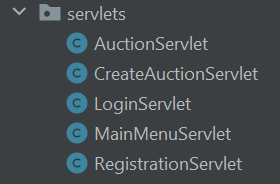
\includegraphics[width=0.4\linewidth]{img/servlets}
 	\caption{}
 	\label{fig:servlets}
 \end{figure}
 

\noindent As shown in the above figure, there is one Java Servlet for each page of the web-application. From the generated page is possible to follow some hyperlinks to find other pages of the web-app.\\
The Webapp folder is organized in the following way:
% TODO: \usepackage{graphicx} required
\begin{figure}[H]
	\centering
	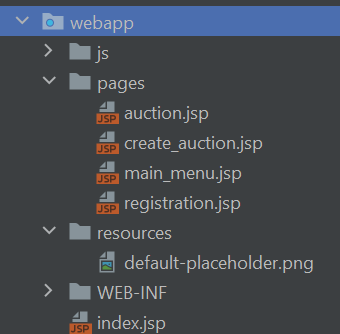
\includegraphics[width=0.4\linewidth]{img/webapp}
	\caption{}
	\label{fig:webapp}
\end{figure}

The actual HTML is generated via JSP technology, with some scriptlets, for each page, in order to have a logic separation between the "View" part and the rest of the application. In example the $main\_menu.jsp$ scriptlet contains some logic to generate different cards by iterating the list of auction returned by the Erlang server.\\

\noindent In order to add some layers of security to the application a couple of Filters were added:\\
% TODO: \usepackage{graphicx} required
\begin{figure}[H]
	\centering
	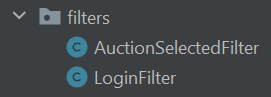
\includegraphics[width=0.4\linewidth]{img/filters}
	\caption{}
	\label{fig:filters}
\end{figure}
\begin{itemize}
	\item \textbf{LoginFilter} is responsible for checking that requests to "protected" pages arrives from users that are already logged in (this can be assured by analyzing the session of the particular user, indexed by a cookie).
		
	\item \textbf{AuctionSelectedFilter} prevents a logged user to access an auction without having pressed the related button. This is done because at the same time multiple auctions can be active at the same time.\\
	
\end{itemize}
In order to update the "Model" part of our application some requests to the Server-Side part in Erlang needs to be done. This is dealt in the communication package:

% TODO: \usepackage{graphicx} required
\begin{figure}[H]
	\centering
	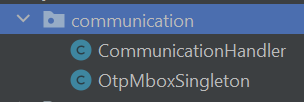
\includegraphics[width=0.4\linewidth]{img/communication}
	\caption{}
	\label{fig:communication}
\end{figure}

\noindent The Jinterface library is used: for each client there is a different mailbox contained in one single "Erlang" node, which is unique since obtained from the session token of the client. Then a request/reply communication happens with the Erlang Main Server or with the related Auction Handler, in case an auction page is requested. The communication will return back a result in order to communicate to the user if the request made has succeeded or not (i.e. a client registration may fail in case of a duplicate username).
\subsection{Web-sockets}
In order to update the application state without requesting periodically a web-page, Web-socket technology is used.

\begin{figure}[H]
	\centering
	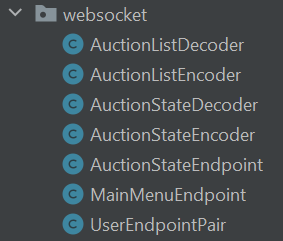
\includegraphics[width=0.4\linewidth]{img/websockets}
	\caption{}
	\label{fig:websockets}
\end{figure}

As we can see in the image above two different web-socket endpoint are used:
\begin{itemize}
	\item \textbf{MainMenuEndpoint}: responsible for updating the state of the main menu w.r.t. the list of active and inactive auctions. Clients connected to this endpoint are registered through the usage of a Java static \textit{CopyOnWriteArraySet} for dealing with concurrent changes of the connected client list.
	\item \textbf{AuctionEndpoint}: responsible for updating the state of the auction w.r.t. the list of joined users, the list of valid bids, the auction time, and the winner election. Clients connected to this endpoint are registered through the usage of a Java static ConcurrentMap$<$String, Set$<$UserEndpointPair$>>$ data structure. With the latter, for each auction name is associated a list of client endpoints. This organization is made in order to correctly send auction messages only to clients that have joined a particular auction, with a publish/subscribe fashion.
\end{itemize}
\subsection{Java Listener}
There's one actor missing in the whole picture: the Java Listener.
The web-socket state update happens with the following sequence of steps:
\begin{enumerate}
	\item A client requests a change to the state of the model (i.e. creates an auction)
	\item Apache Tomcat intercepts the requests and start the communication with the related Erlang server-side which actually stores the application state
	\item The Erlang server-side sends in general \textbf{two messages for each requests}: one is for the servlet itself which acts as an ACK to the request made by the client, one is sent to the \textbf{java listener} for triggering the state change to other clients connected (without need of a page refresh)
	\item Java listener broadcast the state change to all interested users via web-socket
\end{enumerate}  
The advantages of using this approach are the following:
\begin{itemize}
	\item Since messages are sent by the erlang server-side (which actually is the source of truth of the web-application state), the state returned is consistent.
	\item Thanks to web-sockets, there's no need to periodically send request to Apache Tomcat. \textbf{Page updates happens only when there is a state change}, avoiding a considerable amount of computations and HTTP requests to be handled. 
	\item Some events are triggered by erlang side itself and not by the client (i.e. auction ending and winner election), so this approach will update the web-application state correctly by simply avoiding to send one message to Apache Tomcat
\end{itemize}
The \textbf{cost} of this approach is the implementation of the Java Listener.
% TODO: \usepackage{graphicx} required
\begin{figure}[H]
	\centering
	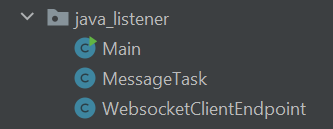
\includegraphics[width=0.4\linewidth]{img/java_listener}
	\caption{}
	\label{fig:javalistener}
\end{figure}

The Java Listener is implemented with a listener Jinterface node for getting requests from Erlang server-side. For handling multiple requests in parallel, threads are used: in particular, for avoiding the overhead due to the creation and termination of threads, \textbf{thread-pooling} is used via ExecutorService instance that implements a fixed thread pool. The task (called MessageTask) computed by each thread is related with sending a message (with the state information) to the correct web-socket endpoint.

\subsection{User Interface} 
In order to ease the UI developing a framework like \textbf{Bootstrap} has been used, in order to create a responsive web-application in a simple way, with a set of ready-to-be-used css classes, without the need of reinventing the wheel by defining our set of css classes for getting the same result. 


A couple of javascript scripts are then defined:

\begin{figure}[H]
	\centering
	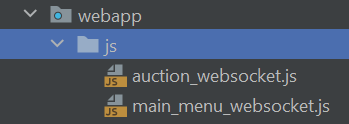
\includegraphics[width=0.4\linewidth]{img/js}
	\caption{}
	\label{fig:js}
\end{figure}

\begin{itemize}
	\item \textbf{main\_menu\_websocket}: Responsible for connecting with the main menu websocket endpoint and to update the DOM of the HTML page when a message arrives.
	\item \textbf{auction\_websocket}: Responsible for connecting the client to the auction websocket endpoint, to update the DOM of the HTML page when a message arrives and to update locally the timer.
\end{itemize}

For what concern form validation, \textbf{browser-default validation} was adopted (i.e. some fields are required to be added, some fields, like the auction duration,  must contain a number).